\scanpage{4}
4) \uline{\unsure{Élargissage}} Opération inverse -- au lieu de
retrancher une couronne, on en rajoute une\ldots

5) Opération mixte : \uline{panachage}

On considère un voisinage tubulaire \unsure{standart|standard}
de $\partial'\widetilde X$, et dans \inserted{chaque composante $T_i$ de} celui-ci, un
cercle $\Gamma_i$, et un isom. rect.
$\Gamma_i\simeq(\partial'\widetilde X)_i$. On \deleted{\unsure{se donne}} \inserted{\deleted{définit}}
\deleted{considère}\inserted{considère} $\deleted{\unsure{\partial}}\widetilde X^{\unsure{*|\circ}}$ déduit de
$\widetilde X$ en enlevant \inserted{$\unsure{K_i}$} ``la \deleted{\unsure{intérieur}}
\deleted{de $\Gamma_i$} partie de $T_i$ entourée
par $\Gamma_i$''. On termine comme dans
3°), 4°) pour trouver $\widetilde X^*$ et $K\subset X^*$.

\figure{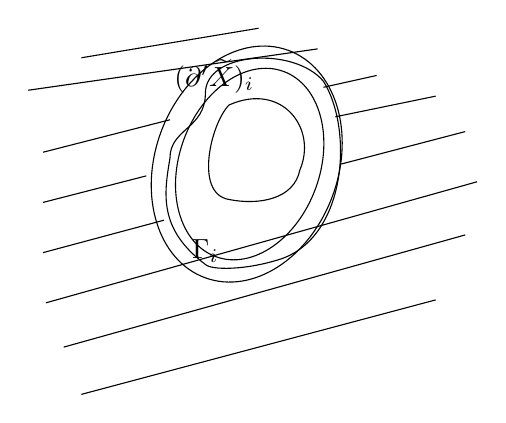
\begin{tikzpicture}[x=.75cm,y=.75cm]
\draw (-2,2.5)--(1,3) (-2.9,1.95)--(2,2.65);
\draw (-2.65,.9)--(-.5,1.45) (2.1,2)--(3.0,2.2);
\draw (-2.65,.05)--(-.9,.5) (2.3,1.5)--(4.0,1.85);
\draw (-2.65,-.8)--(-.6,-.25) (2.4,.7)--(4.5,1.25);
\draw (-2.6,-1.65)--(4.7,.4) (-2.3,-2.4)--(4.5,-.5) (-2,-3.2)--(4,-1.6);
\draw[rotate around={-20:(.8,.7)}] (.8,.7) ellipse (1.55 and 2.05);
\draw[rotate around={-20:(.85,.7)}] (.85,.7) ellipse (1.19 and 1.67);
\draw (.1,-1.0) .. controls (-.7,-.4) and (-.6,.2) .. (-.5,.8)
 .. controls (-.5,1.3) and (.1,1.3) .. (.1,1.9)
 .. controls (.1,2.6) and (1.6,2.7) .. (2.1,2.1)
 .. controls (2.6,1.3) and (2.5,-.5) .. (1.4,-.9)
 .. controls (.8,-1.1) and (.2,-1.1) .. (.1,-1.0);
\draw (.5,.1) .. controls (-.1,.2) and (.2,1.4) .. (.5,1.7)
 .. controls (1.4,2.1) and (2,1.3) .. (1.7,.6)
 .. controls (1.6,.1) and (1,.0) .. (.5,.1);
\node at (.25,2.18) {$(\partial'\widetilde X)_i$};
\node at (.1,-.77) {$\Gamma_i$};
\end{tikzpicture}}

\margin{C'est une composition
rétrécissage $\circ$ élargissage,
ou aussi élargissage $\circ$ rétrécissage.}

\deleted{\unsure{6)}} \uline{\unsure{Commutativité}} de l'opération
de panachage relative à diverses
composantes connexes de $K$.

6) Cas d'une composante \inserted{$C$} de $K$ boucle
isolée \inserted{plongée $\unsure{\mathbb R|\mathbf R}$-analytique}. L'opération de panachage revient
alors tjrs à une composition de 1°) enlever
une couronne \inserted{$\unsure{\mathbb R|\mathbf R}$-analytique}
autour de
$C$ 2°)
Recoller \inserted{$\unsure{\unsure{\mathbb R|\mathbf R}\text{-analytiquement}}$} par
un cylindre les deux
bords \inserted{qui restent} de la couronne
enlevée\ldots

\figure{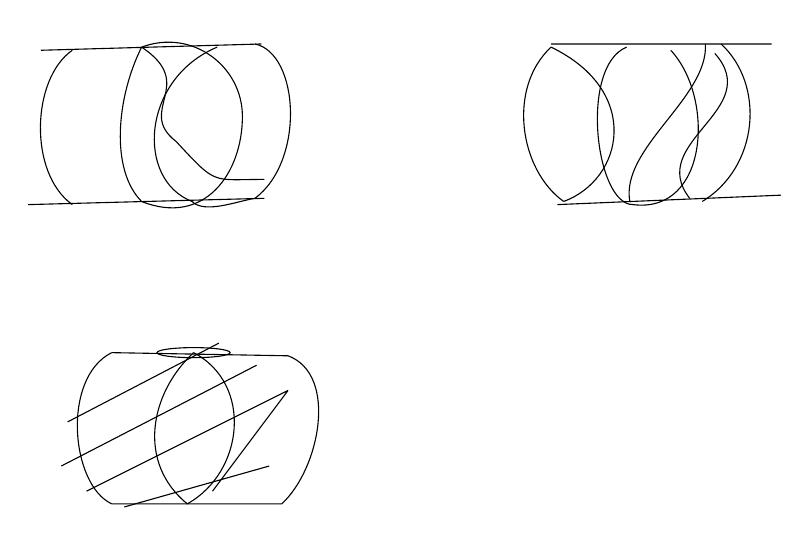
\begin{tikzpicture}[x=.8cm,y=.8cm]
\begin{scope}
\draw (-.4,1.25)--(3.1,1.35) (-.6,-1.2)--(3.15,-1.1);
\draw (.1,1.25) .. controls (-.55,.8) and (-.6,-.7) .. (.1,-1.2);
\draw (3,1.35) .. controls (3.7,1.2) and (3.8,-.5) .. (3,-1.1);
\draw (1.2,1.3) .. controls (.8,.5) and (.7,-.65) .. (1.2,-1.15)
 .. controls (2.2,-1.55) and (2.8,-.7) .. (2.8,.2)
 .. controls (2.8,1) and (2,1.6) .. (1.2,1.3);
\draw (1.2,1.3) .. controls (2.1,.7) and (1.1,.3) .. (1.75,-.2)
 .. controls (2.4,-.9) and (2.3,-.8) .. (3.15,-.8);
\draw (2.4,1.3) .. controls (1.2,.8) and (1.1,-.8) .. (2,-1.15)
 .. controls (2.2,-1.35) and (2.7,-1.15) .. (3,-1.1);
\end{scope}
\begin{scope}[xshift=6.4cm]
\draw (-.3,1.35)--(3.2,1.35) (-.2,-1.2)--(3.35,-1.05);
\draw (-.3,1.3) .. controls (-1.0,.65) and (-.8,-.65) .. (-.1,-1.15);
\draw (-.3,1.3) .. controls (1.15,.6) and (.85,-.8) .. (-.1,-1.15);
\draw (2.4,1.35) .. controls (3.1,.7) and (3,-.6) .. (2.1,-1.15);
\draw (.9,1.3) .. controls (.15,1) and (.4,-1.2) .. (1,-1.2)
 .. controls (2.2,-1.35) and (2.3,.5) .. (1.6,1.25);
\draw (2.15,1.35) .. controls (2.2,.5) and (.8,-.3) .. (.95,-1.15);
\draw (2.3,1.2) .. controls (3.1,.3) and (1.2,-.2) .. (1.9,-1.1);
\end{scope}
\begin{scope}[xshift=.5cm,yshift=-3.8cm]
\draw (.1,1.2)--(2.9,1.15) (.1,-1.2)--(2.8,-1.2);
\draw (.1,1.2) .. controls (-.7,.8) and (-.55,-.9) .. (.1,-1.2);
\draw (2.9,1.15) .. controls (3.7,.85) and (3.4,-.65) .. (2.8,-1.2);
\draw (1.4,1.2) ellipse (.58 and .08);
\draw (1.4,1.2) .. controls (.7,.55) and (.5,-.55) .. (1.3,-1.2)
 .. controls (2.2,-.7) and (2.35,.7) .. (1.4,1.2);
\draw (-.6,.1)--(1.8,1.35) (-.7,-.6)--(2.4,1.0)
 (-.3,-1.0)--(2.9,.6) (1.7,-1.0)--(2.9,.6)
 (.3,-1.25)--(2.6,-.6);
\end{scope}
\end{tikzpicture}}

relations avec les \deleted{\unsure{deux}} \inserted{\unsure{petits}} \unsure{plongements} conformes
d'une petite couronne\ldots
% archive foliation: 3
